%! TEX root = **/report.tex
% vim: spell spelllang=en:

%%%%%%%%%%%%%%%%%%%%%%%%%%%%%%%%%%%%%%%%%%%%%%%%%%%%%%%%%%%%%%%%%%%%%%%%%%%%%%%%
% PREAMBLE
%%%%%%%%%%%%%%%%%%%%%%%%%%%%%%%%%%%%%%%%%%%%%%%%%%%%%%%%%%%%%%%%%%%%%%%%%%%%%%%%
%! TEX root = **/000-main.tex
%%%%%%%%%%%%%%%%%%%%%%%%%%%%%%%%%%%%%%%%%%%%%%%%%%%%%%%%%%%%%%%%%%%%%%%%%%%%%%%%
%% LaTeX preamble, load in main.tex with: \input{preamble}
%%%%%%%%%%%%%%%%%%%%%%%%%%%%%%%%%%%%%%%%%%%%%%%%%%%%%%%%%%%%%%%%%%%%%%%%%%%%%%%%

\documentclass[12pt, oneside]{article}
\usepackage[a4paper, left=2.5cm, right=2.5cm, top=2.5cm, bottom=2.5cm]{geometry}

% for debugging overfulls
%\documentclass[draft, 12pt, oneside]{article}
%\usepackage[showframe, a4paper, left=2.5cm, right=2.5cm, top=2.5cm, bottom=2.5cm]{geometry}

%%%%%%%%%%%%%%%%%%%%%%%%%%%%%%%%%%%%%%%%%%%%%%%%%%%%%%%%%%%%%%%%%%%%%%%%%%%%%%%%
%% FONTS
%%%%%%%%%%%%%%%%%%%%%%%%%%%%%%%%%%%%%%%%%%%%%%%%%%%%%%%%%%%%%%%%%%%%%%%%%%%%%%%%

\usepackage[T1]{fontenc}
\usepackage{fontspec}
\usepackage{microtype}

\setmonofont[Scale=MatchLowercase]{DejaVu Sans Mono}

%%%%%%%%%%%%%%%%%%%%%%%%%%%%%%%%%%%%%%%%%%%%%%%%%%%%%%%%%%%%%%%%%%%%%%%%%%%%%%%%
%% LANGUAGE
%%%%%%%%%%%%%%%%%%%%%%%%%%%%%%%%%%%%%%%%%%%%%%%%%%%%%%%%%%%%%%%%%%%%%%%%%%%%%%%%

\usepackage{polyglossia}
\setdefaultlanguage{english}
\setotherlanguages{spanish,catalan}

%%%%%%%%%%%%%%%%%%%%%%%%%%%%%%%%%%%%%%%%%%%%%%%%%%%%%%%%%%%%%%%%%%%%%%%%%%%%%%%%
%% BIBLIOGRAPHY
%%%%%%%%%%%%%%%%%%%%%%%%%%%%%%%%%%%%%%%%%%%%%%%%%%%%%%%%%%%%%%%%%%%%%%%%%%%%%%%%

\usepackage[
    backend=biber,
    style=numeric,
]{biblatex}
\DeclareNameAlias{default}{family-given}

\addbibresource{biblio.bib}

\usepackage{fvextra}        % Req by minted (must load before csquotes)
\usepackage{csquotes}       % For bibliography quotations
\DeclareQuoteAlias{spanish}{catalan}

%%%%%%%%%%%%%%%%%%%%%%%%%%%%%%%%%%%%%%%%%%%%%%%%%%%%%%%%%%%%%%%%%%%%%%%%%%%%%%%%
%% COMMON
%%%%%%%%%%%%%%%%%%%%%%%%%%%%%%%%%%%%%%%%%%%%%%%%%%%%%%%%%%%%%%%%%%%%%%%%%%%%%%%%

\usepackage{color, xcolor}     % more colors

\usepackage{graphicx}   % graphics
\graphicspath{{./figures/}{../common/}}

\usepackage{comment}

%%%%%%%%%%%%%%%%%%%%%%%%%%%%%%%%%%%%%%%%%%%%%%%%%%%%%%%%%%%%%%%%%%%%%%%%%%%%%%%%
%% MATHS
%%%%%%%%%%%%%%%%%%%%%%%%%%%%%%%%%%%%%%%%%%%%%%%%%%%%%%%%%%%%%%%%%%%%%%%%%%%%%%%%

\usepackage{mathtools}  % amsmath + more
\usepackage{amsthm}     % Theorem enviroment
\usepackage{amssymb}    % More symbols
\usepackage{amstext}    % Text inside mathenv

%\usepackage{relsize}    % Bigger math with mathlarger{___}
%\usepackage{nicefrac}   % nice fractions in one line

%\usepackage{IEEEtrantools} % Complex equation arrays

%%%%%%%%%%%%%%%%%%%%%%%%%%%%%%%%%%%%%%%%%%%%%%%%%%%%%%%%%%%%%%%%%%%%%%%%%%%%%%%%
%% REFERENCES (load order is important)
%%%%%%%%%%%%%%%%%%%%%%%%%%%%%%%%%%%%%%%%%%%%%%%%%%%%%%%%%%%%%%%%%%%%%%%%%%%%%%%%

\usepackage{varioref} % reference far away (1)
\usepackage[colorlinks = true]{hyperref} % links in references (2)
\usepackage{cleveref} % smart references (3)
%hyperref configuration so that it doesn't contrast so much colorlinks,
\hypersetup{
   linkcolor={black},
   citecolor={black},
   %linkcolor={red!50!black},
   %citecolor={blue!50!black},
   urlcolor={blue!80!black}
}

\usepackage[bottom]{footmisc} % Footnotes at bottom of page

%%%%%%%%%%%%%%%%%%%%%%%%%%%%%%%%%%%%%%%%%%%%%%%%%%%%%%%%%%%%%%%%%%%%%%%%%%%%%%%%
%% FIGURES
%%%%%%%%%%%%%%%%%%%%%%%%%%%%%%%%%%%%%%%%%%%%%%%%%%%%%%%%%%%%%%%%%%%%%%%%%%%%%%%%

%\usepackage[export]{adjustbox}  % Adjust table size
\usepackage{float}               % Force tables and images position (H and H!)
%\usepackage{wrapfig}            % Wrap images like in HTML

\usepackage[justification=centering]{caption}
%\usepackage{subcaption}                     % Subfigures
%\usepackage[framemethod=tikz]{mdframed}     % Custom frames

%%%%%%%%%%%%%%%%%%%%%%%%%%%%%%%%%%%%%%%%%%%%%%%%%%%%%%%%%%%%%%%%%%%%%%%%%%%%%%%%
%% TABLES
%%%%%%%%%%%%%%%%%%%%%%%%%%%%%%%%%%%%%%%%%%%%%%%%%%%%%%%%%%%%%%%%%%%%%%%%%%%%%%%%

%\usepackage{colortbl, booktabs} % Better tables
%\usepackage{tabularx}
%\usepackage{longtable} % Multiple page table (does not work with tabularx)
\usepackage{xltabular, colortbl, booktabs} % longtable + tabularx (has bug with booktabs: fix below)

% Split cell in lines and more formating options inside table
\usepackage{array, multirow, multicol, makecell}

%%%
% bug fix for booktabs + xltabular incompatibility
\makeatletter
\def\@BTrule[#1]{%
  \ifx\longtable\undefined
    \let\@BTswitch\@BTnormal
  \else\ifx\hline\LT@hline
    \nobreak
    \let\@BTswitch\@BLTrule
  \else
     \let\@BTswitch\@BTnormal
  \fi\fi
  \global\@thisrulewidth=#1\relax
  \ifnum\@thisruleclass=\tw@\vskip\@aboverulesep\else
  \ifnum\@lastruleclass=\z@\vskip\@aboverulesep\else
  \ifnum\@lastruleclass=\@ne\vskip\doublerulesep\fi\fi\fi
  \@BTswitch}
\makeatother
%%%

%%%%%%%%%%%%%%%%%%%%%%%%%%%%%%%%%%%%%%%%%%%%%%%%%%%%%%%%%%%%%%%%%%%%%%%%%%%%%%%%
%% SIUNITX
%%%%%%%%%%%%%%%%%%%%%%%%%%%%%%%%%%%%%%%%%%%%%%%%%%%%%%%%%%%%%%%%%%%%%%%%%%%%%%%%

%\usepackage[alsoload=hep]{siunitx}          % SI units and uncertainties
%\sisetup{locale = FR}                       % Commas and so on for spanish
%\sisetup{separate-uncertainty=true}
%\sisetup{
  %per-mode=fraction,
  %fraction-function=\nicefrac
%}

%%%%%%%%%%%%%%%%%%%%%%%%%%%%%%%%%%%%%%%%%%%%%%%%%%%%%%%%%%%%%%%%%%%%%%%%%%%%%%%%
%% TIKZ
%%%%%%%%%%%%%%%%%%%%%%%%%%%%%%%%%%%%%%%%%%%%%%%%%%%%%%%%%%%%%%%%%%%%%%%%%%%%%%%%

%\usepackage{tikz}
%\usetikzlibrary{arrows}
%\usetikzlibrary{scopes}
%\usetikzlibrary{babel}

%%%%%%%%%%%%%%%%%%%%%%%%%%%%%%%%%%%%%%%%%%%%%%%%%%%%%%%%%%%%%%%%%%%%%%%%%%%%%%%%
%% MINTED
%%%%%%%%%%%%%%%%%%%%%%%%%%%%%%%%%%%%%%%%%%%%%%%%%%%%%%%%%%%%%%%%%%%%%%%%%%%%%%%%

\usepackage{minted}
\definecolor{codeBg}{HTML}{FFFDE7}
\setminted{
    %style=pastie,
    frame=lines,
    framesep=3mm,
    linenos,
    breaklines=true,
    encoding=utf8,
    fontsize=\footnotesize,
    bgcolor=codeBg
}

%%%%%%%%%%%%%%%%%%%%%%%%%%%%%%%%%%%%%%%%%%%%%%%%%%%%%%%%%%%%%%%%%%%%%%%%%%%%%%%%
%% CUSTOM COMMANDS
%%%%%%%%%%%%%%%%%%%%%%%%%%%%%%%%%%%%%%%%%%%%%%%%%%%%%%%%%%%%%%%%%%%%%%%%%%%%%%%%

% empty whitepage without numbering
\newcommand{\whitepage}{
    \clearpage\thispagestyle{empty}\addtocounter{page}{-1} \newpage \clearpage
}

% Add command before appendix section for page numbering: A-1
\newcommand{\appendixpagenumbering}{
    \break
    \pagenumbering{arabic}
    \renewcommand{\thepage}{\thesection-\arabic{page}}
}

%%%%%%%%%%%%%%%%%%%%%%%%%%%%%%%%%%%%%%%%%%%%%%%%%%%%%%%%%%%%%%%%%%%%%%%%%%%%%%%%
%% CUSTOM MATH OPERATORS (functions not in italic in math mode)
%%%%%%%%%%%%%%%%%%%%%%%%%%%%%%%%%%%%%%%%%%%%%%%%%%%%%%%%%%%%%%%%%%%%%%%%%%%%%%%%

%\DeclareMathOperator{\arcsec}{arcsec}
%\DeclareMathOperator{\arccot}{arccot}
%\DeclareMathOperator{\arccsc}{arccsc}
%\DeclareMathOperator{\cis}{cis}

%%%%%%%%%%%%%%%%%%%%%%%%%%%%%%%%%%%%%%%%%%%%%%%%%%%%%%%%%%%%%%%%%%%%%%%%%%%%%%%%
%% MISC
%%%%%%%%%%%%%%%%%%%%%%%%%%%%%%%%%%%%%%%%%%%%%%%%%%%%%%%%%%%%%%%%%%%%%%%%%%%%%%%%

%\usepackage{datetime} % Customize date
%% \monthyeardate\today gives the date without the day
%\newdateformat{monthyeardate}{%
    %\monthname[\THEMONTH], \THEYEAR}


%%%%%%%%%%%%%%%%%%%%%%%%%%%%%%%%%%%%%%%%%%%%%%%%%%%%%%%%%%%%%%%%%%%%%%%%%%%%%%%%
% EXTRA PACKAGES / CONFIG
%%%%%%%%%%%%%%%%%%%%%%%%%%%%%%%%%%%%%%%%%%%%%%%%%%%%%%%%%%%%%%%%%%%%%%%%%%%%%%%%

\usepackage{tikz}
\usetikzlibrary{shapes,arrows,positioning,calc}
\usetikzlibrary{arrows.meta}
\tikzset{>={Latex[width=3mm,length=3mm]}}

\usepackage{caption}

\usepackage{titling}
\usepackage{cancel}
\usepackage{booktabs}
\usepackage{graphicx}
% Set default figure size
\setkeys{Gin}{width=.9\textwidth, keepaspectratio}

% Center figures by default
\makeatletter
\g@addto@macro\@floatboxreset\centering
\makeatother


%%%%%%%%%%%%%%%%%%%%%%%%%%%%%%%%%%%%%%%%%%%%%%%%%%%%%%%%%%%%%%%%%%%%%%%%%%%%%%%%
% METADATA
%%%%%%%%%%%%%%%%%%%%%%%%%%%%%%%%%%%%%%%%%%%%%%%%%%%%%%%%%%%%%%%%%%%%%%%%%%%%%%%%

% remove when using \maketitle:
% \renewcommand\and{\\[\baselineskip]}

\title{Lab Session 4\\ \Large \normalfont
  MapReduce\\ IRRS
}
\author{
  Aleix Boné
\and
  Marc Maynou
}
\date{Fall 2022}

\setlength{\droptitle}{-5.0em}
% \pretitle{%
% \begin{center}
% \includegraphics[width=0.9\linewidth]{figures/institution-logo.pdf}
% }
% \posttitle{%
% \end{center}
% }

\begin{document}
%%%%%%%%%%%%%%%%%%%%%%%%%%%%%%%%%%%%%%%%%%%%%%%%%%%%%%%%%%%%%%%%%%%%%%%%%%%%%%%%
% TITLE
%%%%%%%%%%%%%%%%%%%%%%%%%%%%%%%%%%%%%%%%%%%%%%%%%%%%%%%%%%%%%%%%%%%%%%%%%%%%%%%%

% Default title or use titlepage.tex

\renewcommand\and{\\[\baselineskip]}
    %! TEX root = **/report.tex
% vim: spell spelllang=en:

\thispagestyle{empty}
\clearpage
\setcounter{page}{-1}

\makeatletter
\begin{titlepage}
{
    \centering
    
\includegraphics[width=0.9\textwidth]{logo-upc-fib}
    \null%
    \vspace{2em}
    {\Huge \bfseries \@title \par}
    \vspace{3em}
    {\large \scshape \@date \par}
    \vspace{2em}
    \vfill
\begin{center}
    % Supplementary image
\end{center}
    \vspace{1em}

    \vfill
    {\raggedleft \large \@author \par}
}
\end{titlepage}
\makeatother


\setlength{\parskip}{1em plus 0.5em minus 0.2em}

%! TEX root = **/report.tex


% DATA: https://github.com/Leixb/IRRS-labs/releases/download/v4.0.0rc/data.tar.gz

% To deliver:
% You will have to deliver a report with the results that you have obtained with the dataset,
% explaining
% how you have generated the datasets,
% what kind of clusters you have found in the data
% and the effect of the size of the vocabulary (number of words selected for representing the documents)
% and the impact of the number of mappers/reducers in the computational cost.
% You can also include in the document the
% main difficulties/choices you had made while implementing this lab session’s

\section*{Introduction}
In this deliverable we will explore the implementation of the \emph{K-Means} algorithm
for clustering similar words through the \emph{MapReduce} computational paradigm.

\section{Implementation}

\subsection{MapReduce KMeansStep.py}

We followed the implementation as outlined in the assignment:

\begin{tikzpicture}[every node/.style={text centered, minimum height=1cm, rectangle, draw}, node distance=0.5cm and 2cm]
    \node (load)  {load\_data};
    \node[right=of load] (assign0)  {assign\_prototype};
    \node[above=of assign0,minimum width=3.7cm] (assign1)  {assign\_prototype};
    \node[draw=none, below=of assign0, node distance=0.1cm and 2cm] (dots)  {$\vdots$};
    \node[below=of dots,minimum width=3.7cm, node distance=0.1cm and 2cm] (assign2)  {assign\_prototype};
    \node[right=of assign0,minimum width=3.7cm] (aggregate)  {\texttt{aggregate\_prototype}};

    \draw[->] (load) -- (assign0);
    \draw[->] (load.10) -- (assign1.west);
    \draw[->] (load.350) -- (assign2.west);
    \draw[->] (assign0) -- (aggregate);
    \draw[->] (assign1.east) -- (aggregate.170);
    \draw[->] (assign2.east) -- (aggregate.190);
\end{tikzpicture}

Where each mapper loads the prototype of each cluster from the provided prototype file and then
computed for each document the Jaccard distance to each prototype. Then it assigns the
prototype with smallest distance to it and emits it to the reducer.

The reducer takes all the documents assigned for each prototype (cluster) and computes the
new prototype from the frequencies of the words in the documents assigned to it.

In our implementation, we used the python data structure \emph{Counter} from the
collections built-in library to efficiently compute the frequencies of the words. This
structure uses a dictionary to store the occurrences of each word.

We considered using two heaps to keep a list of the words and documents sorted as they
are obtained from the mappers. This could theoretically improve the performance
in some cases since we would not have to sort the data at the end of the reducer and
instead the sort is done as the data is obtained. However, we could not justify
this change since the data is not that big and the sorting is not that expensive in our case.

\subsection{MapReduce KMeans.py}

In this script, we performed the background work to run the \emph{KMeans-Step} multiple
times until the prototypes converge.

The only thing we had to do was to save the prototypes in the correct file and format
so that the mappers could load them. And then process the results to check for convergence.

\subsubsection{Convergence}

To check for convergence, our initial approach was to check if the prototypes were the same,
but we quickly realized that floating point precision issues made this approach unreliable.
One workaround we tried was using \emph{numpy.isclose} or \emph{numpy.allclose} to do the
comparison with a small tolerance for numerical errors. This worked but we found that a better
approach was to check if the assigned documents to each consecutive prototype were the same.

To do so, we modified the \emph{KMeans-Step} to emit the list of assigned documents
as well as the prototype for each cluster, then we can check if the set of
assigned documents was the same that the previous prototype. This indicates that the
algorithm has converged.

Another issue was that for some reason, the assigned prototypes swapped names, meaning
that sometimes the cluster 0 would be named 1 and the cluster 1 named 0 in the next iteration.
To solve this, we ignored the cluster names and sorted the list of assigned documents for each
cluster before comparing them.

Given that we had the information of the assigned documents, we decided to saved it into a file
in order to be able to analyze the clusters later.

%! TEX root = **/report.tex
\section{Experimentation}
Once the \emph{K-means} algorithm was fully implemented, we proceeded to test its execution with the \textit{arxiv-abs} dataset.

\subsection{Dataset}

Before trying different parameters and experimenting on the data, we first did a small analysis of the
documents provided.

The dataset of \emph{arxiv-abs} contains 55\,760 documents from 8 different categories. The documents
consist of the abstracts of the papers published in the \emph{arXiv} repository. However, the categories
are not balanced, as shown in \cref{tab:arxiv-abs-categories}. We have to keep this in mind when
analyzing the obtained clusters.

% ls $DATA/arxiv_abs/* | awk 'BEGIN {cnt = 0} $1 ~ ":$" {if (cnt != 0) print cat,cnt; cat = $1; cnt = 0; } {if (cat != $1) cnt++;} END {print cat,
% cnt}' | sed 's#.*/##' | sed 's#\.updates.*:##' | tr ' ' '&'
%
% find  $DATA/arxiv_abs/ -type f -exec wc -w {} \; | \
% sed  's#/.*arxiv_abs/##' counts | sed 's/\.upda.*//' | \
% awk 'BEGIN {sum=0; n=1;} curr!=$2 { print sum,n,sum/n,curr; curr=$2; sum=0; n=0; } { sum+=$1; n++; } END { print sum,n,sum/n,curr}'
\begin{table}[H]
	\begin{threeparttable}[t]
		\caption{Number of documents and average words per document for each category}%
		\label{tab:arxiv-abs-categories}
		\begin{tabular}{llS[table-format=7]S[table-format=5]S[table-format=3.3]}
			\toprule
			{Category}                             & {Abbreviation} & {Documents} & {Total words} & {Avg. words} \\
			\midrule
			Computer Science                       & cs             & 18882       & 5123399       & 271.338      \\
			Astro physics                          & astro-ph       & 13062       & 3679842       & 281.721      \\
			\addlinespace
			Mathematics                            & math           & 6986        & 1900888       & 272.1        \\
			Physiscs                               & physics        & 6847        & 1859268       & 271.545      \\
			Condensed Matter                       & cond-mat       & 5033        & 1350533       & 268.336      \\
			\addlinespace
			Quantum physics                        & quant-ph       & 1876        & 510053        & 271.883      \\
			HEP\tnote{1} \textendash Phenomenology & hep-ph         & 1610        & 442873        & 275.076      \\
			HEP\tnote{1} \textendash Theory        & hep-th         & 1464        & 402725        & 275.085      \\
			\bottomrule
		\end{tabular}
		\begin{tablenotes}
			\item[1] High Energy Physics
		\end{tablenotes}
	\end{threeparttable}
\end{table}

\Cref{tab:arxiv-abs-categories} also shows that the average number of words per document is similar for
all categories, which is to be expected given that the documents are abstracts. We can also see that
there are mainly 3 areas of research: \emph{Computer Science}, \emph{Mathematics} and \emph{Physics}.
The latter with various subcategories, some of which could be very similar to each other (e.g. HEP)

\subsubsection{Zipf}

We took the code from laboratory session 1 and fitted it to the \emph{arxiv-abs} dataset. The results
are shown in \cref{fig:zipf}. As we can see, the data seems to fit Zipf's law, except for the very
few first words and the tail. This is relevant because it means that there are very few words
with high frequency and many words with lower frequency. Latter, we will see that this affects the
size of the vocabulary when setting minimum and maximum frequencies.

\begin{figure}[H]
    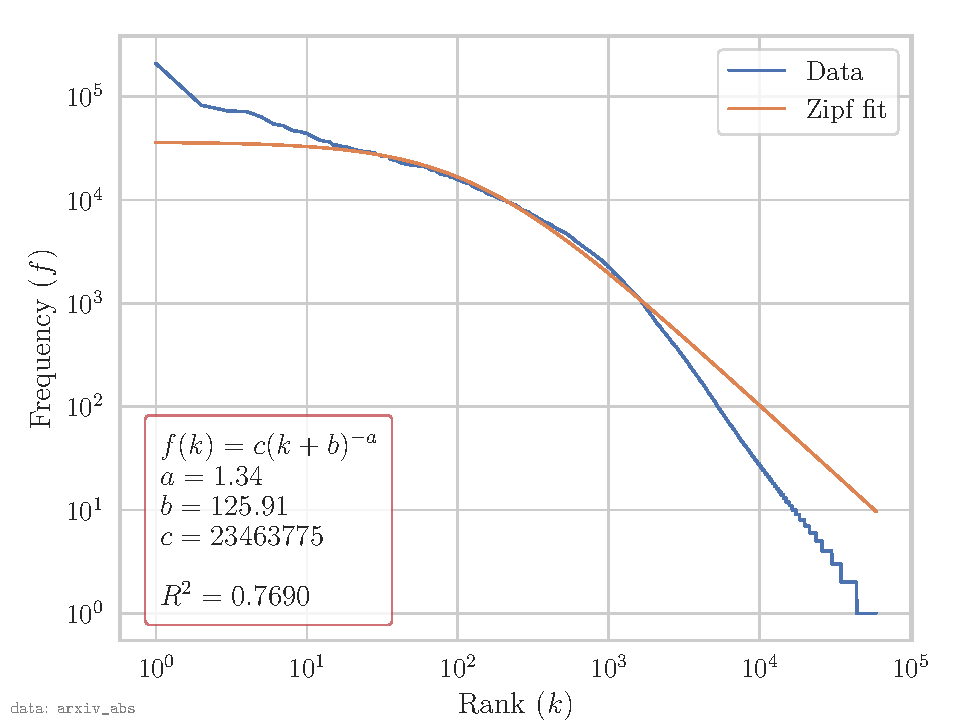
\includegraphics{zipf_loglog}%
    \label{fig:zipf}
    \caption{Zipf plot for the \emph{arxiv-abs} dataset}
\end{figure}

\subsection{Goal}

The clusters obtained using our algorithm heavily depend on the subset of words used to compute
the distances between documents (the vocabulary). If we take words that are common
across all documents, we will find one big cluster with all the documents. If we take words that are
too niche, we will find one cluster per document. Our aim is to find a good balance where
we obtain meaningful clusters from which we can gain some insight.

In the code we have 3 hyper-parameters that determine the words used in the vocabulary:
maximum and minimum frequency (relative to the most common word) and the maximum number
of words. The program will then take all the words with frequencies between the minimum and
the maximum, and if there are more than the $n$ maximum number of words, it will take the $n$
most common words. Note that in this case, the minimum frequency is ignored.

Additionally, we benchmarked the execution time of the algorithm with different number
of processors, to see if the algorithm scales well and estimate the benefits of using
map-reduce parallelization.

\subsection{Implementation}

We departed from the \emph{ExtractData.py} script provided in the laboratory session and modified it
to our needs. We wanted to be able to compute the clusters for different subsets of words by varying
the hyper-parameters outlined in the previous section. To do so, we split the code in two parts,
one that computed the frequencies of all words in the dataset and saved the result into a pickle file.
The second part took the list of parameters and computed the vocabulary and prototype for each valid
combination using the data from the pickle. By doing so we avoid having to recompute the frequencies each
time, and we can also easily parallelize the computation of vocabularies and prototypes.

Finally, we could run the \emph{MRKmeans.py} script for each combination of parameters and
save the result. The results are saved in a plain text file with the full output of the program
which is then parsed using \emph{gnu-awk} to extract the relevant information.

% Similarly, too low a minimum frequency will result in taking too many words, which will make the clusters
% too specific.

\subsection{Vocabulary size}

The first set of experiments was oriented to altering the words used to represent the documents. This is controlled by setting the minimum and maximum values for the frequency of the words selected when executing the system. The following tests were performed by fixing the initial set of clusters to 10 and the maximum number of iterations to 10 as well. We repeated the execution for two sizes of the word set: 100 and 250.

Firstly, we set the minimum frequency to 0, to observe how altering the maximum frequency in isolation could change the execution. The table below presents the results obtained for the set of 100 words:

\begin{table}[H]
	\begin{threeparttable}[t]
		\caption{MapReduce behavior when changing the maximum frequency with a set of 100 words}
		\begin{tabular}{S[table-format=1.2] c c c S[table-format=2.3] S[table-format=1.3]}
			\toprule
			{Max frequency} & Clusters & Iterations \tnote{1} & {\makecell{Total Time         \\ (ms)}} & {\makecell{Avg. iteration time \\ (ms)}} \\
			\midrule
			0.01            & 3        & \textbf{10}          & 29.625                & 2.962 \\
			0.02            & 2        & 3                    & 9.461                 & 3.153 \\
			0.03            & 3        & \textbf{10}          & 34.177                & 3.417 \\
			0.04            & 2        & 3                    & 10.832                & 3.610 \\
			0.05            & 1        & 3                    & 11.524                & 3.841 \\
			0.06            & 3        & \textbf{10}          & 41.341                & 4.134 \\
			0.07            & 1        & 3                    & 14.388                & 4.796 \\
			0.08            & 1        & 3                    & 15.160                & 5.053 \\
			0.09            & 1        & 3                    & 15.571                & 5.190 \\
			\addlinespace
			0.1             & 1        & 4                    & 18.889                & 4.722 \\
			0.2             & 1        & 2                    & 10.597                & 5.298 \\
			0.3             & 1        & 2                    & 11.502                & 5.751 \\
			0.4             & 1        & 2                    & 11.777                & 5.888 \\
			0.5             & 1        & 2                    & 11.567                & 5.783 \\
			0.6             & 1        & 2                    & 11.753                & 5.876 \\
			0.7             & 1        & 2                    & 11.705                & 5.852 \\
			\bottomrule
		\end{tabular}
		\begin{tablenotes}
			\item[1] The iterations are shown in bold when they are the maximum number of iterations (i.e. the algorithm did not converge).
		\end{tablenotes}
	\end{threeparttable}
\end{table}

As it can be seen, for values below 0.07 the execution seems to have an unpredictable behavior, having a convergence rate of 50\%. On the other hand, the number of clusters generated is generally different than 1, which, if our goal is to divide words in groups, seems like a more appropriate choice. From 0.07 we only obtain one cluster by the end of the execution and the algorithm always converges, doing so in just 2 iterations from a maximum frequency of 0.1 onward.

These results are corroborated by the experiments with the word set size of 250, in which considerably similar results were obtained; only differing in the time needed to complete the execution (which makes sense, given that there are more words to process).

Noticing these results, we concluded that the most reasonable value for the maximum frequency should be below 0.1. Values closer to 0 would give a bigger number of clusters while being more unpredictable, whereas values closer to 0.1 would have a more stable execution but the number of clusters would be reduced. We have to take into account that we are using a small number of words, so it is likely that by using a bigger set, the number of clusters would be overall bigger. Nevertheless, this small value helps us to see the effects of altering the frequencies much better.

In order to find reasonable values for the minimum frequency, we executed the algorithm with values of maximum frequency presented before, narrowing the interval to [0.02, 0.1], due to the arguments presented in the previous paragraph. The values for the minimum frequency would be between 0.1 and the maximum frequency (i.e. for maximum frequency = 0.04, we can test minimum frequency values of 0.01, 0.02 and 0.03) and gather the results. Logically, the smaller values would appear in more experiments than the bigger values, so we would average the results to obtain a comparison. We are aware of the possible biases of this approach, but it is still useful to obtain some conclusion. The results are presented in the table below:

\begin{table}[h!]
	\begin{tabular}{c c c c c c}
		\toprule
		Min frequency & Experiments & Clusters & Iterations & Total time & Avg. iteration time \\
		\midrule
		0.01          & 9           & 1.4      & 3.89       & 16.976     & 4.361               \\
		0.02          & 8           & 1.25     & 3.55       & 16.752     & 4.718               \\
		0.03          & 7           & 1.1      & 3.14       & 15.465     & 4.921               \\
		0.04          & 6           & 1.16     & 3.16       & 15.347     & 4.858               \\
		0.05          & 5           & 1.2      & 3.2        & 15.579     & 4.683               \\
		0.06          & 4           & 1.25     & 3.25       & 15.671     & 4.829               \\
		0.07          & 3           & 1.33     & 3          & 14.771     & 4.923               \\
		0.08          & 2           & 1.5      & 3.5        & 14.865     & 4.671               \\
		0.09          & 1           & 1        & 3          & 13.764     & 4.588               \\
		\bottomrule
	\end{tabular}
	\caption{MapReduce behavior when changing the minimum frequency}
\end{table}

When executing these experiments we were expecting the lower values for minimum frequency to generate a higher number of clusters, whereas the bigger values should generate less clusters, given that we are narrowing down the selection of words. Nonetheless, we noticed an interesting pattern, which is that when the minimum frequency got very close to the maximum frequency (e.g. minimum frequency = 0.07 and maximum frequency = 0.08), the number of clusters was generally different than 1, hence the values of the table. We can attribute this to the fact that closing the frequency interval a lot makes the remaining words present enough dissimilarity to generate different clusters. In fact, for most of these cases the number of words was less than the threshold of 100 introduced as a parameter. These results are summarized in the following image:

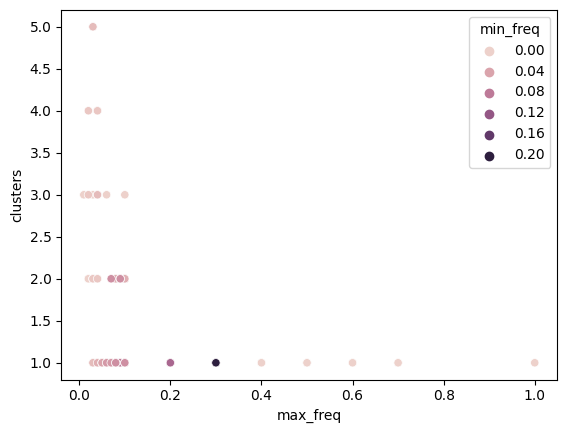
\includegraphics{figures/clusters_per_freq.png}

As for the rest of values of the table, they follow along with the explanation of the previous paragraph: a higher number of clusters implies more iterations to compute them, which requires more time to execute. The results obtained for the set of 250 words presents a similar trend, just with higher cost times. In this latter case, the reduction in the number of words from the 250 threshold is even more noticeable when the frequencies are very close.

As for a final set of ``ideal'' values, we have selected 0.08 and 0.1 as they represent a middle point in between low values (which would result in more clusters but some unexpected behavior) and high values (stable behavior but very similar words).

\subsection{Mappers and Reducers and execution time}

By default, the given script is executed using two mappers and two reducers,
which, a priori, seems inefficient, as a higher number of processes would
complete the execution faster. In order to test this hypothesis, we altered the
\textit{ncores} flag, using values from 1 to 7 and check how this variation
impacted the execution time, doing so for the two word sets generated
beforehand. The maximum number of iterations was fixed to 10, as well as the
initial number of clusters. For each number of cores and for each vocabulary
size 10 executions were triggered, summarizing the average results obtained in
the following tables.

\begin{table}
	\caption{MapReduce behavior when changing the number of cores. Vocabulary size of 100}
    \begin{tabular}{c S[table-format=1.3] S[table-format=2.3] S[table-format=1.3]}
		\toprule
        {Num cores} & {First iteration} & {Total time} & {Avg time per iteration} \\
		\midrule
		1         & 3.565           & 49.102     & 5.455                  \\
		2         & 2.407           & 31.236     & 3.470                  \\
		3         & 2.299           & 26.896     & 2.989                  \\
		4         & 2.229           & 24.834     & 2.760                  \\
		5         & 2.238           & 23.716     & 2.635                  \\
		6         & 2.231           & 23.113     & 2.568                  \\
        \addlinespace
		7         & 2.689           & 27.937     & 3.104                  \\
        \bottomrule
	\end{tabular}
\end{table}

\begin{table}
	\caption{MapReduce behavior when changing the number of cores. Vocabulary size of 250}
    \begin{tabular}{c S[table-format=1.3] S[table-format=3.3] S[table-format=2.3]}
		\toprule
        {Num cores} & {First iteration} & {Total time} & {Avg time per iteration} \\
		\midrule
		1         & 4.429           & 148.248    & 16.472                 \\
		2         & 3.009           & 81.236     & 9.026                  \\
		3         & 2.714           & 60.836     & 6.759                  \\
		4         & 2.591           & 49.904     & 5.544                  \\
		5         & 2.515           & 43.991     & 4.887                  \\
		6         & 2.472           & 39.894     & 4.432                  \\
        \addlinespace
		7         & 2.990           & 50.240     & 5.582                  \\
		\bottomrule
	\end{tabular}
\end{table}

\begin{figure}[H]
    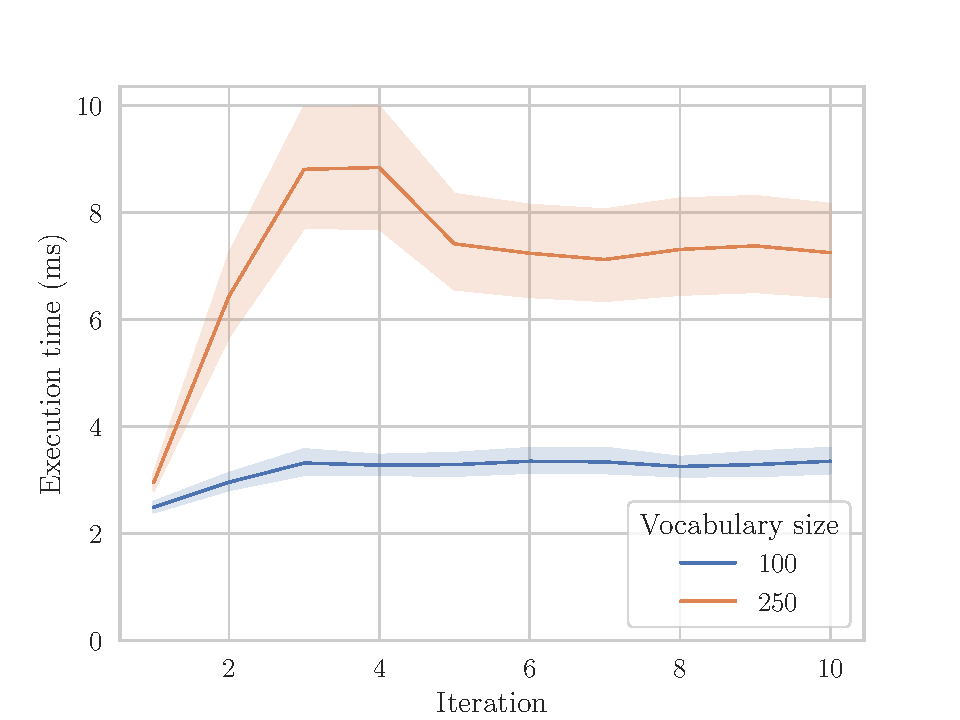
\includegraphics{ex-iter}
    \caption{Execution time for different for each iteration}%
    \label{fig:time-iter}%
\end{figure}

\Cref{fig:time-iter} visualizes the discrepancy between the iteration time of the first
iteration in comparison to the rest (we explain the cause latter).
To prevent it from skewing the results, we excluded it from the visualization
shown in \cref{fig:time-cores}. Where, we can see the results from the previous
tables.

The fact that the first iteration is always considerably quicker than the
others is due to the fact that on this iteration the clusters are
``stored'' in a single document file each. Therefore, the operations needed to calculate
the centroids are more immediate and quicker. For the other iterations, the
centroid needs to be calculated through the documents assigned to each cluster,
which implies a longer list of words to go through, which considerably increases
the time needed to calculate the similarity. We also noticed that the execution
time for the 3rd and 4th iterations of the 250 words vocabulary is considerably
higher than the rest, which may be caused by the fact that the clusters are not
well defined yet and the computation of the centroids are more complex.

\begin{figure}[H]
    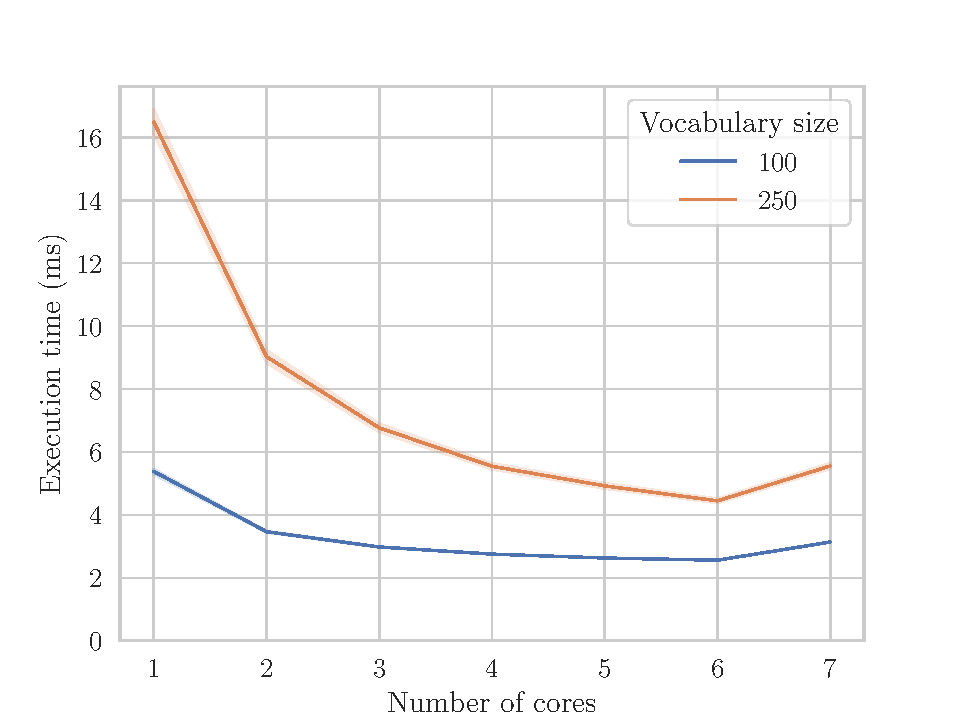
\includegraphics{ex-cores}
    \caption{Execution time for different number of cores 100 and 250 words}%
    \label{fig:time-cores}%
\end{figure}

The first conclusion is that the size of the vocabulary used does impact the
execution time. We can observe that the values of the second table are always
higher than in the first one, which makes sense as the amount of words is more
than doubled. On the other hand, it is clear to see that the more cores used,
the lesser the time needed to execute the whole process. This is specially true
when jumping from 1 to 2 cores, and from 2 to 3. From this point onward the
difference is not that noticeable.

With 7 cores, the execution time increases, this is due to the fact that
the machine where the experiments were executed has 6 cores, and therefore
using more than 6 cores for the computation is detrimental to the performance
since the operating system has to switch between processes.

Notice that the dataset with 250 words shows a stepper decrease in the
execution time, which hints that it parallelizes better than the one with 100.
We can show this by plotting the speedup as a function of the number of cores:

\begin{figure}[H]
    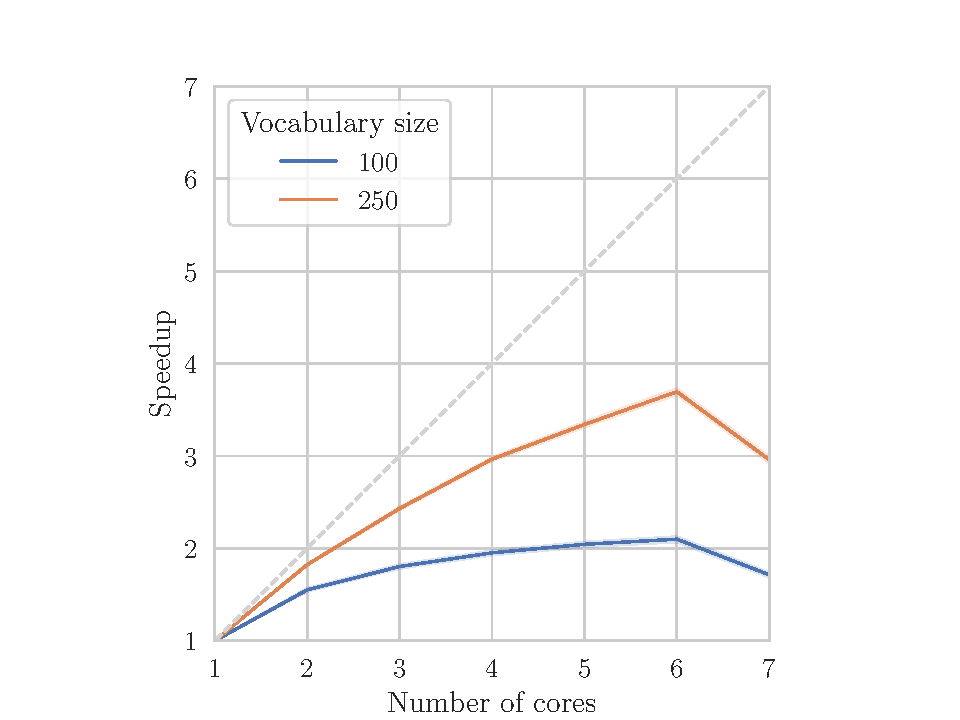
\includegraphics{speedup}
    \caption{Execution time for different number of cores 100 and 250 words}%
    \label{fig:speedup}%
\end{figure}

From \cref{fig:speedup} we can see how the algorithm adheres to the Amdahl's
law, which states that the speedup of a program is limited by the fraction of
serial code in the program. With the dataset of 100 words, we can see that we
are reaching a maximum speedup of around 2.1 and even with our limited
number of cores (6), the speedup is reaching a stable value around 2.2. On the
other hand, with 250 words, the speedup is much higher (3.7) and we cannot appreciate
yet what is the expected maximum speedup. From this we can conclude that with
higher number of words, the parallelizable fraction of the program increases
and thus the speedup is higher, and we benefit more from the MapReduce.

% However, when the number of cores is 7, the time does increase once more. This
% signals that using more cores is not always the best solution. This might seem
% counter-intuitive, as the more cores used, the more the work should be
% distributed and the faster the algorithm should execute. However, we need to
% take into account that there is an additional cost to using more cores, which is
% the overhead required to coordinate and synchronize all the processes. Given the
% results obtained, it would seem that for both vocabulary sized the optimal value
% is 6 cores, as with 7 cores the result gets worse and, presumably, increasing
% the value even more would result in even worse results.


%! TEX root = **/report.tex
\section{Results}

Finally, we took a look at the clusters we obtained with our experimentation. As we have seen,
there are 8 different categories in the dataset but there are some categories that are very broad
and probably can be split into more specific categories. Therefore, we started with 20 clusters.

We run a similar script to the one used on the experiments from the previous sections but using
a more limited search space, a higher number of iterations and 20 clusters as the initial
number of clusters.

The initial expectation was to find clusters that encompassed the subcategories in some
of the bigger and broader categories (mainly computer science and astrophysics). However,
we found that in all the cases where the algorithm converged, there were never
more than 3 clusters.

In the cases where the algorithm did not converge, we found that most of the time
there was one or two clusters that were very large and encompassed most of the
documents, this is a weakness of \emph{K-means}. Even then, they did not have more
than 7 clusters (which is less than the number of categories).

The most interesting results were with the frequency range $[0.08,\, 0.1]$ shown
in \ref{tab:results}. As we can see, the first cluster is much larger and takes
most of the documents from all categories. The other smaller clusters have some dominant categories
such as math, quantum physics and computer science for cluster 2 and astrophysics for cluster 3.

Cluster 3 is the most interesting since it takes a lot of the documents from the astrophysics category
and the only other two categories that are significantly represented are the two from HEP (High energy
physics) which are very related to astrophysics.

\begin{table}[H]
	\caption{Distribution of documents of each category through the cluster}%
	\label{tab:results}%
	\begin{tabular}{lS[table-format=2.2]S[table-format=2.2]S[table-format=2.2]S[table-format=2.2]}
		\toprule
		\multirow{2}{*}{\textbf{Category}} & \multicolumn{4}{c}{\textbf{Cluster}}                        \\
		                                   & {1}                                    & {2}   & {3}   & {4}  \\
		\midrule
		% astro-ph & 7414   & 311    & 4395   & 939    \\
		% cond-mat & 4451   & 265    & 15     & 300    \\
		% cs       & 15909  & 1979   & 14     & 963    \\
		% hep-ph   & 1308   & 82     & 111    & 108    \\
		% hep-th   & 1282   & 66     & 40     & 71     \\
		% math     & 5525   & 1056   & 12     & 370    \\
		% physics  & 5709   & 565    & 50     & 518    \\
		% quant-ph & 1562   & 223    & 2      & 86     \\
		astro-ph                           & 56.77                                  & 2.38  & 33.65 & 7.19 \\
		cond-mat                           & 88.47                                  & 5.27  & 0.30  & 5.96 \\
		cs                                 & 84.33                                  & 10.49 & 0.07  & 5.10 \\
		hep-ph                             & 81.29                                  & 5.10  & 6.90  & 6.71 \\
		hep-th                             & 87.87                                  & 4.52  & 2.74  & 4.87 \\
		math                               & 79.35                                  & 15.17 & 0.17  & 5.31 \\
		physics                            & 83.44                                  & 8.26  & 0.73  & 7.57 \\
		quant-ph                           & 83.40                                  & 11.91 & 0.11  & 4.59 \\
		\bottomrule
	\end{tabular}
\end{table}

In \cref{tab:vocabulary} we show some of the words that are used in this execution (out of 100). We can
see that there are some field specific words such as ``galaxy'' and ``neural'' but also other
more generic words such as ``best'', or ``common''.

\begin{table}[H]
	\caption{Vocabulary for frequency range $[0.08,\, 0.1]$ (top 20)}%
	\label{tab:vocabulary}%
	\begin{tabular}{rl}
		\toprule
		Occurrences & Word     \\
		\midrule
		4946        & select   \\
		4946        & constant \\
		4920        & neural   \\
		4912        & shown    \\
		4879        & address  \\
		4857        & key      \\
		4824        & spatial  \\
		4769        & art      \\
		4745        & reveal   \\
		4723        & us       \\
		\bottomrule
	\end{tabular}
	\hspace{2em}
	\begin{tabular}{rl}
		\toprule
		Occurrences & Word    \\
		\midrule
		4722        & open    \\
		4710        & galaxi  \\
		4704        & complet \\
		4675        & part    \\
		4665        & finit   \\
		4642        & best    \\
		4639        & contain \\
		4632        & probabl \\
		4628        & common  \\
		4604        & signal  \\
		\bottomrule
	\end{tabular}
\end{table}

% data/arxiv_abs_30/100_0.08_0.1/vocabulary.txt

% data/arxiv_abs_30/100_0.04_0.07/vocabulary.txt


\section*{Conclusions}

We have implemented a MapReduce \emph{K-means} for documents in Python and tested it
with the \emph{arXiv-abs} dataset. We have found that the algorithm is
parallelizable using map-reduce and that the higher the size of the vocabulary, the
better it parallelizes. The algorithm is very sensitive to the set of words
used for computing the distances. Despite trying lots of different ranges of word frequencies it
we did not converge to more than 3 clusters in any case.

This is probably due to the fact that the method of choosing the words from the frequency list
is not the best one since it is difficult to isolate words related to specific fields of study.
Other metrics such as \emph{TF-IDF} could be used to improve the results.

%\pagebreak
% \null
% \vfill
% \printbibliography
\end{document}
